\documentclass[conference,12pt]{IEEEtran}

\usepackage[tight,footnotesize]{subfigure}

\usepackage{algorithmic}
\usepackage[boxed]{algorithm}

\usepackage{mathtools}

\usepackage[pdftex]{graphicx}
\graphicspath{{./images/}}

\hyphenation{op-tical net-works semi-conduc-tor}

\begin{document}

\title{\vspace{-0.05\textheight}System Design Project - Final Report}

\author{\vspace{-0.05\textheight}\IEEEauthorblockN{Marc Howarth}
\IEEEauthorblockA{Group 12 - Robot Unicorn Defenders}}
	
\maketitle

\IEEEpeerreviewmaketitle

\section{Introduction}
Given the challenge of designing a Lego robot that could play football was a daunting one. From the outset, it was apparent a project of this scale would require a great deal of organisation. Setting up a Google Group and a wiki\footnote{https://sites.google.com/site/edisdp12/} helped keep the group well communicated but none of our ideas materialised until Joe stepped forward as project manager and split the group into four sub-teams.
\begin{itemize}
\item Construction
\item Movement and Strategy
\item Simulator
\item Vision
\end{itemize}
I spent the majority of my time working with the Movement and Strategy team but also helped the Vision team at various points throughout the project.

In order to give ourselves the best chance of winning it was decided to build a fast robot. Watching videos of the previous matches on YouTube it was apparent that the first robot to the ball first was often the robot who eventually scored. With this in mind the team set out, with a winning mindset, to build an agile, lightweight robot.

\section{Code Structure}
The decision to use LeJOS was made swiftly at the start of the project, allowing work on the code to begin as soon as possible. The software, NXT-G, installed on the brick by default was to be replaced with LeJOS because:
\begin{itemize}
\item LeJOS is a Java based system, a programming language that all the group were comfortable using.
\item Eclipse can have various LeJOS features integrated into it's interface.
\item Previous SDP years used LeJOS, leaving plenty of documentation to look through.
\end{itemize}

A persistent Bluetooth connection had to be established between a PC and the brick to allow continuous control of the robot. A client - server system was drawn up, testing the ability to successfully transmit a command from a PC (server) which the robot (client) could understand and execute accordingly.

In an attempt to send as much information as possible over the Bluetooth connection we experimented sending strings over the data stream however, for reasons still unknown to us, LeJOS would always crash on receiving a string. Sending integers one at a time worked consistently and led to a protocol being set up between the client and server:
\begin{itemize}
\item 0: \textit{EXIT}: Close Bluetooth connection.
\item 1: \textit{KICK}: activate the kicker once.
\item 2: \textit{MOVE}: rotate left/right wheel x/y amount.
\item 3: \textit{ROTATE}: rotates x degrees.
\item 4: \textit{STOP}: stop all motors.
\item 5: \textit{CELEBRATE}: activate a celebration song.
\item 6: \textit{PENALTY}: take a penalty.
\end{itemize}
In order to read the parameters - \textit{x} for ROTATE and \textit{x,y} for MOVE - the client knew to read additional integers from the data stream before retrieving any proceeding commands.

\section{Movement}
The biggest milestone for the movement sub-team was getting the robot to approach the ball. This was the first challenge that required all parts of our project to be successfully integrated and running in a continuous loop. Algorithm 1 shows the first attempt at getting to the ball.

\begin{algorithm}
\caption{GoToBall}
\begin{algorithmic}[1]
\WHILE {UpdateVision()}
	\STATE $threshold\gets 30$
	\STATE $distance\gets distanceFromBall()$
	\STATE $dAngle\gets robotAngle() - angleToBall()$
	\IF{$dAngle<0$ \AND $\|dAngle\|<180$ \OR $dAngle>180$ \AND $\|dAngle\|>180$}
		\STATE $right \gets -1$
		\STATE $left \gets 1$
	\ELSE
		\STATE $right \gets 1$
		\STATE $left \gets -1$
	\ENDIF
	\IF{$\|dAngle\| < threshold$}
		\STATE $right \gets distance$
		\STATE $left \gets distance$
	\ENDIF
	\STATE rotateWheels($right$, $left$)
\ENDWHILE
\end{algorithmic}
\end{algorithm}

The robot has three options: rotate left, rotate right, or go forwards at a speed proportional it's distance from the ball. When developing this algorithm, poor orientation calculation was compensated for by using a threshold of 30 degrees. It was tempting to decrease this threshold to increase the speed at which the robot approached the ball, however with thresholds less than 30 degrees the robot continually rotated left and right without ever going forwards.

Until the orientation calculations from the vision team were more precise, this algorithm was used until milestone 3. After the third milestone the focus moved onto working with potential fields as a method of getting from A to B. Potential fields, uses a velocity vector calculated from attraction forces (usually from a destination point) and repulsive forces (such as an opponent) which is then translated into independent wheel speeds. Having independent wheel speeds immediately presents an advantage over the previous method allowing the robot to travel in an arc.

The majority of the work towards potential fields was completed by Behzad however I helped with the initial testing and tweaking of values to get the algorithm working well on the pitch. Problems that arose in the first versions of potential fields were
\begin{itemize}
\item Velocity vectors were too large, and when translated into wheel speeds gave values $>$2000. The maximum wheel rotate speed for our robot was 500.
\item Robot slowed to almost a stop when 10cm from the destination.
\item Erratic turning e.g. turning 270 degrees left instead of 90 degrees right.
\end{itemize}
The stopping distance and large vectors were fixed by testing various values of the \textit{power} and \textit{influence distance} of the attraction vector. Erratic turning was a little harder to correct but after debugging, it was noticeable that the angular velocity (calculated from the final velocity) was not being normalised between $-\pi$ and $\pi$ properly.

Potential fields allowed to us to move extremely quickly around the pitch, being faster than all our opponents at approaching the ball at the start of a match. Unfortunately, the potential fields path planning had no concepts of walls. Thus, even though the destination point may be within the pitch boundaries, the calculated path may not be contained inside the pitch and result in our robot driving into the wall. Given more time we would have liked to have given every wall a repulsive force such that the robot could smoothly approach the wall when required.

Two touch sensors were mounted at the front of the robot allowing the robot to adjust if it hit the wall or the opponent. The robot adjusting allowed the path planning the change its route however sometimes it would take up to three attempts at driving into the wall before finding a better path.

\section{Strategy}
Getting the ball away from the wall proved to be problem in our friendly matches, whenever the ball was near the wall the robots often had to be reset back to initial positions. To avoid this, a strategy was developed to kick the ball towards the wall in the direction of the opponent's goal. Figure \ref{fig:rebound} shows the required rebound point, the equations below give x,y coordinates of rebound point.
\[y = \left\{ 
\begin{array}{l l}
  0 & \quad \mbox{ballY $<$ 155}\\
  310 & \quad \mbox{otherwise}\\ \end{array} \right. \]
\[x = \frac{ballX(goalY-y) + goalX(ballY-y)}{ballY + goalY - 2y} \]
In solving these equations the angle of entry and exit of the ball are assumed to be equal. This assumption worked perfectly when testing the strategy on the simulator however, through tests on the pitch, if the ball had lost speed before hitting the wall the rebound angle was dramatically reduced and the ball remained close to the wall. 

To ensure the ball the ball approached the wall with enough speed, the GetBallFromWall strategy was only ever activated when the ball was 30 pixels\footnote{All distances were measured as pixels based on images captured from the video feed} away from the wall. Adjusting the equations to be more precise is very hard as it would require taking into consideration the spin of the ball, frictional coefficients of both objects and the coefficient of restitution. The simple model proved effective at getting the ball back into open play and occasionally scored a goal.

\section{Penalty}
As a smaller robot, we often were award multiple penalties in the matches. To utilise this, a method for taking penalties was hard-coded onto the robot. The ball position and robot position remained constant for every penalty, therefore it was possible to calculate the exact angle of rotation to ensure the ball was aimed towards the corner of the opponent goal $>$90\% of the time. Problems with hard-coding methods into the robot arose when the construction team changed the robot design.

Most the construction changes towards the end of the project were minimal however, late on, it was decided to replace the robot's caster wheel with a ball bearing. In doing so, gave the robot more weight, stability and balance allowing testing of potential fields at higher speeds. The inclusion of the ball bearing meant that the accuracy of a hard-coded penalty was dramatically decreased. When repeating penalties from the same spot, the ball would only travel towards the corner of the goal 20\% of the time.

The advantages of the ball bearing outweighed the lack of penalty accuracy. For the final match, the main strategy was initiated immediately after taking the penalty and so if the penalty was not scored, the robot could quickly take advantage of the fact that the ball was close to the opponent's goal.

\section{Initial Attack}
To fully exploit our speed, an initial attack was set up to ensure that the robot was always first to the ball from the starting positions. Figure \ref{fig:initial1} shows the points drawn by the strategy at the start of a match. The optimal point is placed behind the ball at a distance, \textit{optimalGap}, to allow room for rotation before approaching the ball.

Potential fields will decrease in speed as it approaches it's destination, therefore having an intermediary point, \textit{optimum}, meant the robot would slow down when reaching optimum then pick up speed to reach the ball. This is clearly an inefficient method of attacking the ball. A variable, \textit{initial}, was introduced and set to \textit{true} whenever a strategy was reset. Implementing Algorithm 2 allowed a rapid, smooth approach to the ball; Figure \ref{fig:initial2} demonstrates updated positions when using the initial attack.

\begin{algorithm}
\caption{Initial Attack}
\begin{algorithmic}[1]
\STATE $initial\gets true$
\WHILE {UpdateVision()}
	\IF{$initial$}
		\IF{isRobotNearBall()}
			\STATE $optimalGap\gets 30$
		\ELSE
			\STATE $optimalGap\gets 120$
			\STATE $inital\gets false$
			\STATE kick()
		\ENDIF
	\ENDIF
\ENDWHILE
\end{algorithmic}
\end{algorithm}

\section{Conclusion}
This project was my first experience in collaborating on a large scale assignment, it gave a hands on approach to ideas that I had personally only theorised before, such as coding standards and the use of Javadoc. Having never used version control before, I am now using it for personal projects and various assignments from other classes.

Looking back at the start of the project, various awkward meetings and conversations with people who barely knew each other, our group worked well together. A vital ingredient in the making of our lean mean goal scoring machine.\footnote{Full credit to Calum Jackson for the creation of this phrase}

\newpage

\section{Appendix}

\begin{figure}[htp]
\begin{center}
\leavevmode
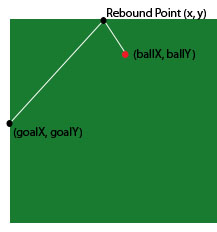
\includegraphics[width=0.4\textwidth] {rebound.jpg}
\end{center}
\caption{Rebound Point}
\label{fig:rebound}
\end{figure}

\begin{figure}[htp]
\begin{center}
\leavevmode
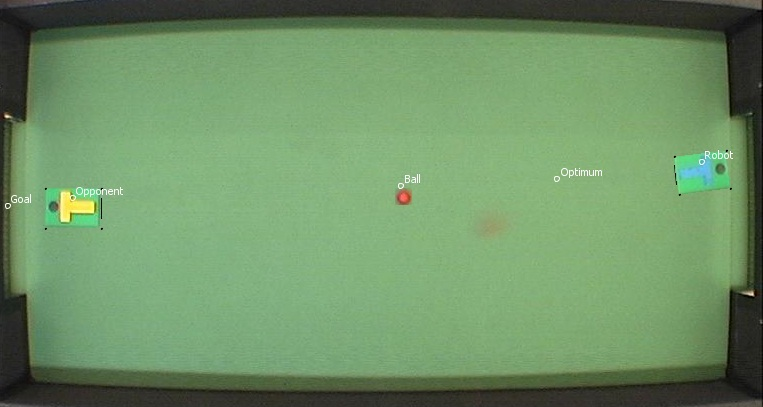
\includegraphics[width=0.8\textwidth] {initial1.jpg}
\end{center}
\caption{Initial Positions}
\label{fig:initial1}
\end{figure}

\clearpage 

\begin{figure}[htp]
\begin{center}
\leavevmode
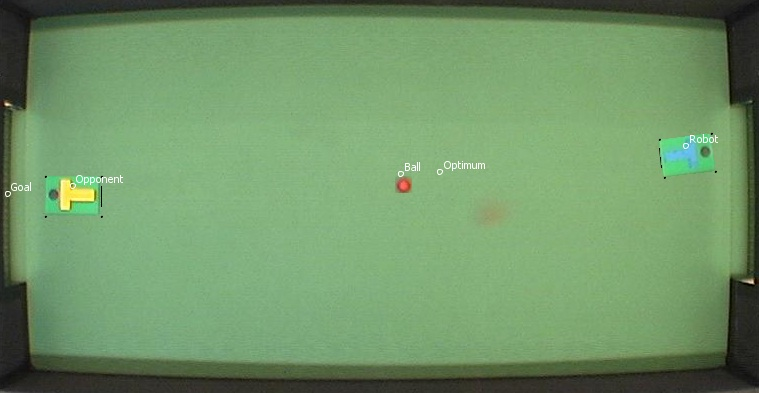
\includegraphics[width=0.8\textwidth] {initial2.jpg}
\end{center}
\caption{Initial Postions with Attack}
\label{fig:initial2}
\end{figure}

\end{document}